%# -*- coding: utf-8 -*-
%%采用 xelatex + ctex 文档类
\documentclass[fancyhdr,fntef,UTF8,oneside,12pt,a4paper, winfonts]{ctexbook}
%%%%%!!!请将您的个人信息按照注释正确填写!!!%%%%%

%%%%%封面及摘要内容,中文 
\newcommand{\department} {软件学院}  	%院系
\newcommand{\major}      {软件工程} 	%专业方向
\newcommand{\thesistitle}{基于Javascript的词法分析器自动生成工具 —— Alice Lex} 	%论文题目
\newcommand{\grade}      {2012}	    %年级
\newcommand{\NJUID}      {081251041}%学号
\newcommand{\myname}     {葛羽航}		%姓名
\newcommand{\advisor}    {葛季栋}		%指导老师姓名
\newcommand{\advisorjob} {讲师}		%指导老师职称
\newcommand{\enteryear}  {2008}		%入学年份

%%%%%封面及摘要内容,英文
\newcommand{\edepartment} {Software Institute}	%院系
\newcommand{\emajor}      {Software Engineering}				%专业方向
\newcommand{\ethesistitle}{A Lexical Analyzers Automatic Generator - Alice Lex}			%论文题目
\newcommand{\emyname}     {Yuhang Ge}			%姓名
\newcommand{\eadvisor}    {Jidong Ge}				%指导老师姓名
% !Mode:: "TeX:UTF-8"
%% 字体设置
\setCJKfamilyfont{song}{SimSun}
\setCJKfamilyfont{zhongsong}{STZhongsong}
\setCJKfamilyfont{kai}{KaiTi}
\setCJKfamilyfont{hei}{SimHei}
\setCJKfamilyfont{fs}{FangSong}
\setCJKfamilyfont{li}{LiSu}
\setCJKfamilyfont{yy}{YouYuan}
\newcommand{\song}{\CJKfamily{song}}
\newcommand{\zs}{\CJKfamily{zhongsong}}
\newcommand{\kai}{\CJKfamily{kai}}
\newcommand{\hei}{\CJKfamily{hei}}
\newcommand{\fs}{\CJKfamily{fs}}
\newcommand{\li}{\CJKfamily{li}}
\newcommand{\yy}{\CJKfamily{yy}}
\setmainfont{Times New Roman} %英文字体使用Times New Roman
%\setmainfont[SmallCapsFont=LMRomanCaps10]{Times New Roman}
%Times New Roman 字体不包括 Small Caps 形状,如果要使用,需设定 Small Caps 字体,如 LMRomanCaps10

\renewcommand{\ULthickness}{0.7pt}
\newcommand{\myuline}[2]      {\uline{\makebox[#1]{#2}}}
\newcommand{\NJUTunderline}[1]{\uline{\hfill{#1}\hfill}}
\footnotesep=10pt

\usepackage{amsmath,amsfonts,amssymb}
\usepackage{array}
\usepackage{booktabs,multirow,colortbl,longtable}
\usepackage{verbatim}
\usepackage{lipsum}
\usepackage{comment}
\usepackage{footnpag}

%% 加载图形宏包
\usepackage{graphicx}
%% 设置图片目录
\graphicspath{{figures/}}
\usepackage[config]{subfig}
\usepackage{indentfirst}
\usepackage[neverdecrease]{paralist}
\let\itemize\compactitem
\let\enditemize\endcompactitem
\let\enumerate\compactenum
\let\endenumerate\endcompactenum
\let\description\compactdesc
\let\enddescription\endcompactdesc

%%设置浮动体(表格、图片)标题格式
\DeclareCaptionLabelFormat{nju}{{\zihao{5}\song #1~#2}}
\DeclareCaptionLabelSeparator{nju}{\hspace{1em}}
\DeclareCaptionFont{nju}{\zihao{5}\song}
\captionsetup{labelformat=nju,labelsep=nju,font=nju}
\captionsetup[table]{position=top,belowskip={12bp-\intextsep},aboveskip=6bp}
\captionsetup[figure]{position=bottom,belowskip={12bp-\intextsep},aboveskip=6bp}

%% 超链接、目录
\usepackage{hyperref}
\usepackage{xcolor}
\definecolor{darkblue}{rgb}{0,0,0.55}
\hypersetup{CJKbookmarks,bookmarksnumbered,%
			colorlinks,unicode=true,%
			linkcolor=black,%
			citecolor=darkblue,%
			plainpages=false,%
			bookmarksopen=true,%
			bookmarksopenlevel=1,
			pdfstartview=FitH,
			pdftitle={\thesistitle},
    		pdfauthor={\myname},
    		pdfcreator={XeLaTeX with NJUThesis template designed by pkuphy},}
\usepackage{tabularx}%只要把tabularx包的引用放到hyperref包之后,正文脚注编号就能正常生成超链接。
%%版面控制
\usepackage{geometry}
\geometry{top=3.5cm,bottom=3.5cm,left=3.2cm,right=3.2cm}
%\geometry{headheight=2.6cm,headsep=5mm,footskip=13mm}
\parskip 0.5ex plus 0.25ex minus 0.25ex

\renewcommand{\textfraction}{0.15}
\renewcommand{\topfraction}{0.85}
\renewcommand{\bottomfraction}{0.65}
\renewcommand{\floatpagefraction}{0.60}


\fancypagestyle{myfancy}{%
\fancyhf{}
\fancyhead[C]{\small \song\leftmark}
\fancyfoot[C]{\small \thepage}
\renewcommand{\headrulewidth}{0.7pt}
}
\pagestyle{myfancy}


\setcounter{secnumdepth}{3}%%自动编号到 subsubsection

\CTEXsetup[nameformat={\hei\zihao{-2}}]{chapter}
\CTEXsetup[titleformat={\hei\zihao{-2}}]{chapter}
\CTEXsetup[beforeskip={-20pt}]{chapter}
\CTEXsetup[afterskip={20pt}]{chapter}
\CTEXsetup[format={\hei\zihao{-3}}]{section}
\CTEXsetup[nameformat={\bf\hei\zihao{-3}}]{section}
\CTEXsetup[beforeskip={-3ex plus -1ex minus -.2ex}]{section}
\CTEXsetup[afterskip={1.0ex plus .2ex}]{section}
\CTEXsetup[format={\hei\zihao{-4}}]{subsection}
\CTEXsetup[nameformat={\bf\hei\zihao{-4}}]{subsection}
\CTEXsetup[beforeskip={-2.5ex plus -1ex minus -.2ex}]{subsection}
\CTEXsetup[afterskip={1.0ex plus .2ex}]{subsection}
\CTEXoptions[contentsname={目\qquad 录}]
\CTEXoptions[listfigurename={插\qquad 图}]
\CTEXoptions[listtablename={表\qquad 格}]

%% 中文破折号,来自清华模板
\newcommand{\pozhehao}{\kern0.3ex\rule[0.8ex]{2em}{0.1ex}\kern0.3ex}

\newenvironment{abstract}{
\thispagestyle{plain}
\pagenumbering{Roman}
\pdfbookmark[0]{����ժҪ}{abstract}
\begin{center}
{\bf\kai\zihao{-2} \uuline{��~��~��~ѧ~��~��~��~��~ҵ~��~��~��~��~ժ~Ҫ}}
\end{center}
\bigskip

\noindent
\begin{minipage}{\textwidth}
\kai\zihao{4}%
\noindent{��ҵ������Ŀ��}\NJUTunderline{\thesistitle}\\
\NJUTunderline{\department}{Ժϵ}\NJUTunderline{\major}{רҵ}
\NJUTunderline{\enteryear}{��������}\hfill{������}\NJUTunderline{\myname}\\
{ָ����ʦ��������ְ�ƣ���}\uline{\hfill\advisor ��\advisorjob\hfill}
\end{minipage}

\vskip 1cm
\begin{center}
{\heiti\zihao{-3} ժ\quad Ҫ}
\end{center}\par
\kai\zihao{-4}
}{}
\newcommand\keywords[1]{\vspace{2ex}\noindent{\hei �ؼ��ʣ�} {\kai #1}}

\newenvironment{englishabstract}{
\clearpage
\thispagestyle{plain}
\pdfbookmark[0]{Ӣ��ժҪ}{englishabstract}
\begin{center}
{\bf\kai\zihao{-2} \uuline{��~��~��~ѧ~��~��~��~��~ҵ~��~��~Ӣ~��~ժ~Ҫ}}
\end{center}
\bigskip

\noindent
{\zihao{4}%
\begin{description}
\item{THESIS:} {\bf\ethesistitle}
\item{DEPARTMENT:} {\bf\edepartment}
\item{SPECIALIZATION:} {\bf\emajor}
\item{UNDERGRADUATE:} {\bf\emyname}
\item{MENTOR:} {\bf\eadvisor}
\end{description}
}
\vskip 1cm
\begin{center}
{\bf\zihao{-3} Abstract}
\end{center}\par
}{}
\newcommand\englishkeywords[1]{\vspace{2ex}\noindent{\bf Keywords:} #1}

\renewcommand\maketitle{%
\clearpage
\thispagestyle{empty}
\pdfbookmark[0]{封面}{cover}

\begin{center}
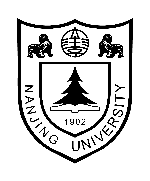
\includegraphics[width=1.96cm]{logo} \\
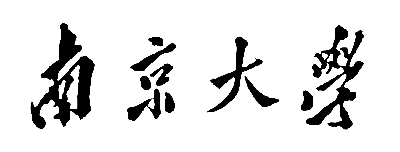
\includegraphics[height=2cm]{name} \\
\vskip 1cm
\zs
\zihao{0} 本~~科~~毕~~业~~论~~文\\
\vskip 2in\zihao{3}
\begin{minipage}{0.9\textwidth}
院\qquad 系\NJUTunderline{\department}\\[3mm]
专\qquad 业\NJUTunderline{\major}\\[3mm]
题\qquad 目\NJUTunderline{\thesistitle}\\[3mm]
年\qquad 级\myuline{4.5cm}{\grade}{\hfill}学\qquad 号\myuline{4cm}{\NJUID}\\[3mm]
学生姓名\NJUTunderline{\myname}\\[3mm]
指导老师\myuline{4.5cm}{\advisor}{\hfill}职\qquad 称\myuline{4cm}{\advisorjob}\\[3mm]
论文提交日期\NJUTunderline{\today}
\end{minipage}
\end{center}
\clearpage
\thispagestyle{empty}
\vspace*{\stretch{1}}
{\kai\zihao{-3}
\noindent
\begin{tabular}{ccr}
\begin{CJKfilltwosides}{3.5cm}学号\end{CJKfilltwosides} & : & \makebox[6cm][r]{\NJUID}\\
\begin{CJKfilltwosides}{3.5cm}论文答辩日期\end{CJKfilltwosides} & : & \uline{\qquad}年\uline{\quad}月\uline{\quad}日\\
\begin{CJKfilltwosides}{3.5cm}指导教师\end{CJKfilltwosides} & : & \uline{\qquad\qquad\quad}(签字)\\
\end{tabular}
}
}

\newcommand\makeenglishtitle{%
\clearpage
\thispagestyle{empty}
\begin{center}
\vspace*{20pt}
\bf\zihao{2} \ethesistitle
\vskip \stretch{1}
\normalfont\zihao{4} by
\vskip 3pt
\bf\zihao{4} \emyname
\vskip \stretch{1}
\normalfont\zihao{4} Directed by
\vskip 3pt
\bf\zihao{4} \eadvisor
\vskip \stretch{2}
\normalfont\large \edepartment \\Nanjing University
\vskip 30pt
\CTEXoptions[today=old]
\normalfont\large \today
\vskip 20pt
\it\large Submitted in full fulfilment of the requirements\\for the degree of Bachelor of Science in Xxx.
\end{center}
}


\begin{document}
\maketitle
\makeenglishtitle
\frontmatter
\normalfont
\begin{abstract}
本文是南京大学本科学位论文的\LaTeX 模板。\par

 褐蚁已经忘记这里曾是它的家园。这段时光对于暮色中的大地和刚刚出现的星星来说短得可以忽略不计,但对于它来说却是漫长的。\par
在那个已被忘却的日子里,它的世界颠覆了。泥土飞走,出现了一条又深又宽的峡谷,然后泥土又轰隆隆地飞回来,峡谷消失了,在原来峡谷的尽头出现了一座黑色的孤峰。其实,在这片广阔的疆域上,这种事常常发生,泥土飞走又飞回,峡谷出现又消失,然后是孤峰降临,好像是给每次灾变打上一个醒目的标记。褐蚁和几百个同族带着幸存的蚁后向太阳落下的方向走了一段路,建立了新的帝国。\par
\end{abstract}

\keywords{\LaTeX ;南京大学}

\begin{englishabstract}
\lipsum[1]
\end{englishabstract}
\englishkeywords{NJUthesis template}
\clearpage

\pdfbookmark[0]{目录}{tableofcontents}
\tableofcontents
\listoffigures
%\listoftables  这条命令是表格目录,需要的话可以启用;上面那条是图片目录,不需要可以注释掉或者直接删除

\mainmatter
\zihao{-4}
\song
\chapter{������}
\label{cha:intro}
��һ�½���һЩ������ \LaTeX ����������塢��ѧ��ʽ�����񡢲�ͼ���ο����׵ȡ�

\section{����}
�����������ο� \verb|cover.tex| �����������dz��򵥣�һ�����ᡣ
������������Ŀ����ʦ����ְ�Ƶ���Ϣ�� \verb|name.tex| �У��Լ���һ�¡�

\section{����}
\begin{center}
\begin{tabular}{lc}
\verb|\song| & \song ����\\
\verb|\kai|  & \kai  ����\\
\verb|\hei|  & \hei  ����\\
\verb|\fs|   & \fs   ����\\
\verb|\li|   & \li   ����\\
\verb|\yy|   & \yy   ��Բ\\
\verb|\zs|   & \zs   ����\\
\end{tabular}
\end{center}

������������Ӵ�Ч�����ÿ������û����������塣
��������������������ӻ��������������壺\\
\url{https://jianguoyun.com/c/pubfile/Lye3gYc3po3MwHB-Cd2j9Vj-3EH6MG1XbiAmcxZzvak}
\section{��ѧ}
�Լ��ұ��鿴�ɡ��Ƽ� lshort �� lnotes ��������\\
\url{http://www.dralpha.com/chs/tech/lnotes2.pdf}\\
\url{http://ftp.ctex.org/mirrors/CTAN/info/lshort/chinese/lshort-zh-cn.pdf}

\section{����}
�Լ��ұ��鿴�ɡ�

\section{��ͼ}
��ͼ���
\begin{verbatim}
\begin{figure}[http]
\centerline{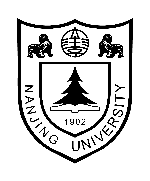
\includegraphics[width=1.97cm]{logo}}
\caption{�Ͼ���ѧУ��}
\label{fig:logo}
\end{figure}
\end{verbatim}

\begin{figure}[htbp]
\centerline{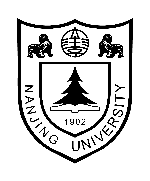
\includegraphics[width=1.97cm]{logo}}
\caption{�Ͼ���ѧУ��}
\label{fig:logo}
\end{figure}

\begin{figure}[htbp]
\centerline{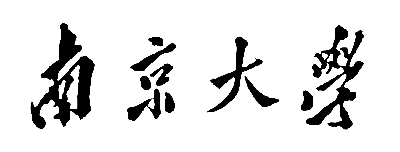
\includegraphics[height=2cm]{name}}
\caption{�Ͼ���ѧë��У��}
\label{fig:name}
\end{figure}


\section{�����}
Casting Metal Nanowires Within Discrete Self-Assembled Peptide Nanotubes{\cite{casting}}

Blue Luminescence Based on Quantum Confinement at Peptide Nanotubes{\cite{qc}}

\section{���뷽��}
���� \texttt{xelatex} ���룬���̣�
\begin{verbatim}
xelatex main
bibtex  main
xelatex main
xelatex main
\end{verbatim}
���� Linux �û�����д�˸��򵥵� \texttt{Makefile}���ڵ�ǰĿ¼�ն������� \texttt{make} ���ɡ�


\chapter{地球往事}

\section{三体二}

\subsection{序章}
……

孤峰上的褐蚁本来想转向向上攀登,但发现前面还有一道凹槽,同在“7”
之前爬过的那个它喜欢的形状“9”一模一样,它就再横行过去,爬了一遍这个
“9”。它觉得这个形状比“7”和“1”好,好在哪里当然说不清,这是美感的原
始单细胞态;刚才爬过“9”时的那种模糊的愉悦感再次加强了,这是幸福的原
始单细胞态。但这两种精神的单细胞没有进化的机会,现在同一亿年前一样,同
一亿年后也一样。

“小罗啊,冬冬常提起你,她说你是……搞天文学的?”

“以前是,现在我在大学里教社会学,就在您那所学校,不过我去时您已经
退休了。”

“社会学,跨度这么大?”

“是,杨冬总说我这人心很散。”

“哦,怪不得她说你很聪明的。”

“小聪明而已,和您女儿不在一个层次。只是感觉天文专业是铁板一块,在
哪儿钻个眼儿都不容易;而社会学之类的是木板,总能找些薄的地方钻透的,比
较好混吧。”

抱着再遇到一个“9”的愿望,褐蚁继续横行,但前面遇到的却是一道直直
的与地面平行的横槽,好像是第一道槽横放了,但它比“1”长,两端没有小细
槽,呈“---”状。

“不要这么说,这是正常人的生活嘛,都像冬冬那样怎么行。”

“我这人确实胸无大志,很浮躁的。”

“我倒是有个建议:你为什么不去研究宇宙社会学呢?”

“宇宙社会学?”

“我随便说的一个名词,就是假设宇宙中分布着数量巨大的文明,它们的数
目与能观测到的星星是一个数量级的,很多很多,这些文明构成了一个总体的宇
宙社会,宇宙社会学就是研究这个超级社会的形态。”

孤峰上的褐蚁继续横向爬了不远,期望在爬过形状为“---”的凹槽后再找到
一个它喜欢的“9”,但它遇到的是“2”。这条路线前面部分很舒适,但后面的急
转弯像前面的“7” 一样恐怖,似乎是个不祥之兆。褐蚁继续横爬,下一道凹槽是
一个封闭的形状:“0”。这种路程是“9”的一部分,但却是一个陷阱:生活需要
平滑,但也需要一个方向,不能总是回副起点,褐蚁是懂这个的。虽然前面还有
两道凹槽,但它已失去了兴趣,转身向上攀登。

“可……目前只知道我们这一个文明啊。”

“正因为如此没有人去做这个事情,这就留给你一个机会嘛。”

“叶老师,很有意思!您说下去。”

“我这么想是因为能把你的两个专业结合起来,宇宙社会学比起人类社会学
来呈现出清晰的数学结构。”

“为什么这么说呢?”

叶文洁指指天空,西方的暮光仍然很亮,空中的星星少得可以轻易数出来。
这很容易使人回想起一个星星都没有出现时的苍穹,那蓝色的虚空透出一片广阔
的茫然,仿佛是大理石雕像那没有瞳仁的眼睑。现在尽管星星很稀少,这巨大的
空跟却有了瞳仁。于是空虚有了内容,宇宙有了视觉。但与空间相比,星星都是
这么微小,只是一个个若隐若现的银色小点,似乎暗示了宇宙雕刻者的某种不安
——他(它)克服不了给宇宙点上瞳仁的欲望,但对宇宙之眼赋予视觉又怀着某种
巨大的恐惧,最后,宅间的巨大和星星的微小就是这种欲望和恐惧平衡的结果,
昭示着某种超越一切的谨慎。

“你看,星星都是一个个的点,宇宙中各个文明社会的复杂结构,其中的混
沌和随机的因素,都被这样巨大的距离滤去了,那些文明在我们看来就是一个个
拥有参数的点,这在数学上就比较容易处理了。”

“但,叶老师,您说的宇宙社会学没有任何可供研究的实际资料,也不太可
能进行调查和实验。”

“所以你最后的成果就是纯理论的,就像欧氏几何一样,先设定几条简单的
不证自明的公理,再在这些公理的基础上推导出整个理论体系。”

“叶老师,这……真是太有意思了,可是宇宙社会学的公理是什么呢?”
“第一,生存是文明的第一需要;第二,文明不断增长和扩张,但宇宙中的
物质总量保持不变”

褐蚁向上爬了不远,才知道上方也有凹槽,而且是一堆凹槽的组合,结构像
迷宫般复杂。褐蚁对形状是敏感的,它自信能够搞清这个形状,但为此要把前面
爬过的那些形状都忘掉,因为它那小小的神经网络存贮量是有限的。它忘掉“9”
没有感到遗憾,不断地忘却是它生活的一部分,必须终身记住的东西不多,都被
基因刻在被称做本能的那部分存贮区了。

清空记忆后,它进入迷宫,经过一阵曲折的爬行,它在自己简陋的意识中把
这个形状建立起来:“墓”。再向上,又是一个凹槽的组合,但比前一个简单多了,
不过为了探索它,褐蚁仍不得不清空记忆,忘掉“墓”。它首先爬进一道线条优
美的槽,这形态让它想起了不久前发现的一只刚死的蝈蝈的肚子。它很快搞清了
这个结构:“之”。以后向上的攀登路程中,又遇到两个凹槽组合。前一个中包括
两个水滴状的坑和一个蝈蝈肚子——“冬”;最上面的一个分成两部分,组合起
来是“杨”。这是褐蚁最后记住的一个形状,也是这段攀登旅程中唯一记住的一
个,前面爬过的那些有趣的形状都忘掉了。

“叶老师,从社会学角度看,这两条公理都是足够坚实的……您这么快就说
出来,好像胸有成竹似的。”罗辑有些吃惊地说。

“我已经想了大半辈子,但确实是第一次同人谈起这个,我真的不知道为什
么要谈……哦,要想从这两条公理推论出宇宙社会学的基本图景,还有两个重要概
念:猜疑链和技术爆炸。”

“很有意思的两个名词,您能解释一下吗?”

叶文洁看看表:“没有时间了,其实你这样聪明,自己也能想出来,你可以
先从这两条公理着手创立这门学科,那你就有可能成为宇宙社会学的欧几里得
了。”

“叶老师,我成不了欧几里得,但会记住您的话,试着去做做,以后我可能
还会去请教您。”

“怕没有机会了……或者,体就当我随便说说,不管是哪种情况,我都尽了责
任。好,小罗,我走了。”

“……叶老师,您保重。”

叶文洁在暮色中离去,走向她那最后的聚会。

褐蚁继续攀登,进入了峭壁上的一个圆池,池内光滑的表面上有一个极其复
杂的图像,它知道自己那小小的神经网络绝对无力存贮这样的东西,但了解了图
像的大概形状后,它又有了对“9”的感觉,原细胞态的美感又萌动了一下。而
且它还似乎认出了图像中的一部分,那是一双眼睛,它对眼睛多少有一些敏感,
因为被眼睛注视就意味着危险。不过此时它没有什么忧虑,因为它知道这双眼睛
没有生命。它已经忘记了那个叫罗辑的巨大的存在在第一次发出声音前蹲下来凝
视孤峰上端的情形,当时他凝视的就是这双眼睛。接着,它爬出圆池,攀上峰顶。
在这里。它并没有一览众山小的感觉,因为它不怕从高处坠落,它曾多次被风从
比这高得多的地方吹下去,但毫发无损,没有了对高处的恐惧就体会不到高处之
美。

在孤峰脚下,郡只被罗辑用花柄拂落的蜘蛛开始重建蛛网,它从峭壁上拉出
一根晶莹的丝,把自己像钟摆似的甩到地面上。这样做了三次,网的骨架就完成
了。网被破坏一万次它就重建一万次,对这过程它没有厌烦和绝望,也没有乐趣,
一亿年来一直如此。

罗辑静立了一会儿,也走了。当地面的震动消失后,褐蚁从孤峰的另一边向
下爬去,它要赶回蚁穴报告那只死甲虫的位置。天空中的星星密了起来,在孤峰
的脚下,褐蚁又与蜘蛛交错而过,它们再次感觉到了对方的存在,但仍然没有交
流。

褐蚁和蜘蛛不知道,在宇宙文明公理诞生的时候,除了那个屏息聆听的遥远
的世界,仅就地球生命而言,它们是仅有的见证者。\cite{threebody}

\section{黑暗森林理论}


两人走到了公路的另一侧,这里,路基挡住了居民区的灯光,四周漆黑一片,
罗辑和史强摸索着坐在沙地上。
\marginparwidth=17mm
\marginpar{\kai\textcolor{red}{尼玛不要把最精华的部分透露出来好不好啊!}}

“我们开始吧。”罗辑的声音在黑暗中响起。

“你讲通俗点儿。我这文化水平,复杂了听不懂。”

“谁都能懂。大史,真理是简单的,它就是这种东西,让你听到后奇怪当初
自己怎么就发现不了它。你知道数学上的公理吗?”

“在中学几何里学过,就是过两点只能划一根线那类明摆着的东西。”

“对对,现在我们要给宇宙文明找出两条公理:一、生存是文明的第一需要。
二、文明不断增长和扩张,但宇宙中的物质总量保持不变。”

“还有呢?”

“没有了。”

“就这么点儿东西能推导出什么来?”

“大史,你能从一颗弹头或一滴血还原整个案情,宇宙社会学也就是要从这
两条公理描述出整个银河系文明和宇宙文明的图景。科学就是这么回事,每个体
系的基石都很简单。”

“那你推导一下看看?”

“首先我们谈谈黑暗战役的事,如果我说星舰地球是宇宙文明的缩影,你相
信吗?”

“不对吧,星舰地球缺少燃料和配件这类资源,但宇宙不缺,宇宙太大了。”

“你错了,宇宙是很大,但生命更大!这就是第二条公理所表明的。宇宙的
物质总量基本恒定,但生命却以指数增长!指数是数学中的魔鬼,如果海中有一
个肉眼看不到的细菌,半小时分裂一次,只要有足够的养料,几天之内它的后代
就能填满地球上所有的海洋。不要让人类和三体世界给你造成错觉,这两个文明
是很小,但它们只是处于文明的婴儿阶段,只要文明掌握的技术超过了某个阈值,
生命在宇宙中的扩张是很恐怖的。比如说,就按人类目前的航行速度,一百万年
后地球文明就可以挤满整个银河系。一百万年,按宇宙尺度只是很短的时间啊。”

“你是说,从长远来看,全宇宙也可能出现星舰地球那样的...他们怎么说来
着,生存死局?”

“不用从长远看,现在整个宇宙已经是一个生存死局了!正像希恩斯所说,
文明很可能几十亿年前就在宇宙中萌发了,从现在的迹象看,宇宙可能已经被挤
满了,谁也不知道银河系和整个宇宙现在还有多少空地方,还有多少没被占用的
资源。”\footnote{不同生命性质的文明间需占有不同的资源,所以宇宙文明的资源分配可
能分成相互平行的很多层次,从碳基生命、硅基生命直至恒星生命和电磁生命,
所需的资源基本包括了宇宙间所有的物质形态,各层所涉及的资源大部分互不
干扰,但也有重叠。}

“这也不对吧?宇宙看上去空荡荡的,除了三体,没有看到别的外星生命
啊?”

“这是我们下面要说的,给我一支烟。”罗辑摸索了半天才从大史手中拿到
烟,再听到罗辑说话时,史强发现他已经坐到离自己有三四米远的地方了,“我
们得拉开点距离。才更有太空的感觉。”罗辑说,然后,他拧动香烟的过滤嘴部
分,把烟点燃了,同时,史强也点上了一支烟。黑暗中,两颗小火星遥遥相对。
“好,为了说明问题,现在我们需要建立一个最简洁的宇宙文明模型:这两
个火星就代表两个文明星球,整个宇宙只由这两个星球组成,其他什么都没了,
你把周围的一切都删除。怎么样,找到这个感觉了吗?”

“嗯,这感觉在这种黑地方比较好找。”

“现在我们分别把这两个文明世界称做你和我的文明,两个世界相距遥远,
就算一百光年吧。你探测到了我的存在。但不知道更详细的情况,而我完全不知
道体的存在。”

“嗯。”

“下面要定义两个概念:文明问的善意和恶意。善和恶这类字眼放到科学中
是不严谨的,所以需要对它们的含义加以限制:善意就是指不主动攻击和消灭其
他文明,恶意则相反。”

“这是最低的善意了吧?”

“你已经知道了我这个文明在宇宙中的存在,下面就请考虑你对于我有什么
选择。请注意,这个过程中要时刻牢记宇宙文明公理,还要时刻考虑太空中的环
境和距离尺度。”

“我选择与你交流?”

“如果这样做,你就要注意自己付出的代价:你暴露了自己的存在。”

“是,这在宇宙中不是一件小事。”

“有各种程度的暴露:最强的暴露是使我得知你在星际的精确坐标,其次是
让我知道你的大致方向,最弱的暴露是仅仅让我得知你在宇宙中的存在。但即使
是最弱的暴露也有可能使我搜索并找到你。既然你能够探知我的存在,我当然也
有可能找到你,从技术发展角度看,这只是个时间问题。”

“可老弟,我可以冒一下险与你交流,如果你是恶意的,那算我倒霉;如果
你是善意的,那我们就可以进一步交流,最后联合成一个更大的善意文明。”

“好,大史,我们到了关键之处。下面再回到宇宙文明公理上来:即使我是
善意文明,我是否能够在交流开始时就判断休也是善意的呢?”

“当然不行,这违反第一条公理。”

“那么,在我收到你的交流信号后,我该怎么办?”

“你当然应该首先判断我是善意还是恶意,如果是恶意,你消灭我;如果是
善意,我们继续交流。”

罗辑那边的火星升了起来并来回移动,显然是他站起身来踱步,“在地球上
是可以的,但在宇宙中不行,下面我们引入一个重要概念:猜疑链。”

“挺怪的词儿。”

“我开始仅得到这么一个词,她没有解释,但我后来终于从字面上推测出了
它的含义。”

“他?他是谁?”

“……后面再说吧,我们继续:如果你认为我是善意的,这并不是你感到安全
的理由,因为按照第一条公理,善意文明并不能预先把别的文明也想成善意的,
所以,你现在还不知道我是怎么认为你的,你不知道我认为你是善意还是恶意;
进一步,即使你知道我把你也想象成善意的,我也知道你把我想象成善意的,但
是我不知道你是怎么想我怎么想你怎么想我的,挺绕的是不是?这才是第三层,
这个逻辑可以一直向前延伸,没完没了。”

“我懂你的意思。”

“这就是猜疑链。这种东西在地球上是见不到的。人类共同的物种、相近的
文化、同处一个相互依存的生态圈、近在咫尺的距离,在这样的环境下,猜疑链
只能延伸一至两层就会被交流所消解。但在太空中,猜疑链则可能延伸得很长,
在被交流所消解之前,黑暗战役那样的事已经发生了。”

大史抽了一口烟,他沉思的面容在黑暗中显现了一下,“现在看来黑暗战役
真的能教会我们好多事。”

“是的,星舰地球的五艘飞船仅仅是五个‘类宇宙文明’,还不是真正的宇
宙文明——因为它们都是由人类这同一物种组成的,相互间的距离也很近——尽
管这样,在生存死局下,猜疑链还是出现了。而在真正的宇宙文明中,不同种族
之间的生物学差异可能达到门甚至界一级,
\footnote{在生物学上,生物分头分为界、门、纲、目、科、属、种,阶层越是往
下,彼些之间特征就越相似。地球人类的种族之间在生物学上的差异也就局限
于种这一层级,如果考虑到非碳基生命的存在,外星种族的差异可能超越了界
一级。}
文化上的差异更是不可想象,且
相隔着无比遥远的距离,它们之间猜疑链几乎是坚不可摧的。”

“这就是说,不管你我是善意文明还是恶意文明,结果都一样?”

“是的,这就是猜疑链最重要的特性:与文明本身的社会形态和道德取向没
有关系,把每个文明看成链条两端的点即可,不管文明在其内部是善意的还是恶
意的,在进入猜疑链构成的网络中后都会变成同一种东西。”

“可是如果你比我弱小很多呢,对我没有威胁,这样我总可以和你交流吧?”

“也不行,这就要引人第二个重要概念:技术爆炸。这个概念她也没来得及
说明,但推测起来比猜疑链要容易得多。人类文明有五千年历史,地球生命史长
达几十亿年,而现代技术是在三百年时间内发展起来的,从宇宙的时间尺度上看,
这根本不是什么发展,是爆炸!技术飞跃的可能性是埋藏在每个文明内部的炸药,
如果有内部或外部因素点燃了它,轰一下就炸开了!地球是三百年,但没有理由
认为宇宙文明中人类是发展最快的,可能其他文明的技术爆炸更为迅猛。我比你
弱小,在收到你的交流信息后得知了你的存在,我们之间的猜疑链就也建立了,
这期间我随时都可能发生技术爆炸,一下子远远走在你的前面,变得比你强大。
要知道在宇宙尺度上,几百年只是弹指一挥间,而我得知你的存在和从交流中得
到的信息,根可能是技术爆炸最好的导火线。所以,即使我仅仅是婴儿文明或萌
芽文明,对你来说也是充满危险的。”

史强看着远处罗辑那边黑暗中的火星想了几秒钟,又看看自己的烟头,“那,
我只能保持沉默了。”

“你想想这对吗?”

他们都抽着烟,随着火星不时增亮,两个面容交替在黑暗中浮现,仿佛是这
个简洁宇宙中两个深思的上帝。

史强说:“也不行,如果你比我强大,既然我能发现你,那你总有一天能搜
寻到我,这样我们之间就又出现了猜疑链;如果你比我弱小,但随时可能发生技
术爆炸,那就变成第一种情况了。总结起来,一、让你知道我的存在;二、让你
存在下去,对我来说都是危险的,都违反第一条公理。”

“大史,你真的是个头脑很清楚的人。”

“这一开始我的脑瓜还是能跟上你的。”

罗辑在黑暗中沉默了很长时间,他的脸在火星的微光中浮现了两三次,才说:

“大史,不是什么开始,我们的推论已经结束了。”

“结束?我们什么也没弄出来呀?你说的宇宙文明图景呢?”

“你在得知我的存在后。交流和沉默都不行,你也只剩一个选择了。”

在长时间的沉默中,两个火星都熄灭了,没有一丝风,黑暗在寂静中变得如
沥青般黏稠,把夜空和沙漠糊成一体。最后,史强只在黑暗中说出一个字:

“操!”

“把你的这种选择外推到千亿颗恒星中的亿万文明上,大图景就出来了。”

罗辑在黑暗中点点头说。

“这……也太黑了吧……”

“真实的宇宙就是这么黑。”罗辑伸手挥挥,像抚摸天鹅缄般感受着黑暗的
质感,“宇宙就是一座黑暗森林,每个文明都是带枪的猎人,像幽灵般潜行于林
间,轻轻拨开挡路的树枝,竭力不让脚步发出一点儿声音,连呼吸都小心翼翼……
他必须小心,因为林中到处都有与他一样潜行的猎人。如果他发现了别的生命,
不管是不是猎人,不管是天使还是魔鬼,不管是娇嫩的婴儿还是步履蹒跚的老人,
也不管是天仙般的少女还是天神般的男神,能做的只有一件事:开枪消灭之。在
这片森林中,他人就是地狱,就是永恒的威胁,任何暴露自己存在的生命都将很
快被消灭。这就是宇宙文明的图景,这就是对费米悖论的解释。”

%% !Mode:: "TeX:UTF-8"
\chapter{结论}
\section{Conclusion}
\lipsum[87]

\begin{figure}
\centerline{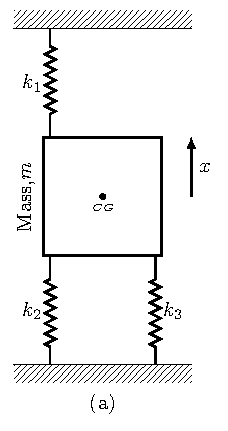
\includegraphics[scale=1.5]{tikzspring.pdf}}
\caption{弹簧}
\label{fig:spring}
\end{figure}

\backmatter
\pagenumbering{Roman}
% 参考文献
\bibliographystyle{unsrt}
\bibliography{ref/reference}
\addcontentsline{toc}{chapter}{参考文献}
% 致谢
% !Mode:: "TeX:UTF-8"
\chapter*{致\qquad 谢}
\addcontentsline{toc}{chapter}{致谢}

感谢国家,感谢父母,感谢老师,感谢……

\end{document}